\documentclass[12pt, final]{article}
\usepackage{color}
\usepackage{times}
\usepackage{amssymb,amsmath,amsthm}
\usepackage{comment}
\usepackage{dsfont}
\usepackage{graphicx}
\usepackage{enumerate}
\usepackage{enumitem}
\usepackage[paperwidth=8.5in,left=1.0in,right=1.0in,top=1.0in,bottom=1.0in,paperheight=11.0in]{geometry}
\usepackage[labelsep=colon,singlelinecheck=false,footnotesize]{caption}
\usepackage{fancyhdr}
\usepackage{float}
\usepackage{booktabs}
\usepackage[sort&compress]{natbib}
\usepackage{subfig}
\usepackage{titlesec}
\usepackage[breaklinks]{hyperref}
\hypersetup{pdfdisplaydoctitle=true,bookmarksnumbered=true,colorlinks=true,citecolor=black,linkcolor=darkblue,urlcolor=darkred,pdfstartview=FitH,pdfpagemode=UseNone}
\usepackage[hyphenbreaks]{breakurl}
\usepackage{accents}
\newcommand{\ubar}[1]{\underaccent{\bar}{#1}}


%Define Color Names
\definecolor{Gray}{rgb}{0.65,0.65,0.65}
\definecolor{darkblue}{rgb}{0,0,0.55}
\definecolor{darkred}{rgb}{0.5,0,0}

%Section Headings
\newcommand\Bheadfont{\fontsize{14pt}{\baselineskip}\selectfont}
\titleformat{\section}[hang]{\normalfont\sc\color{darkblue}\Bheadfont}{\thesection\hskip0.618em}{0em}{}
\titlespacing*{\section}{0pt}{15pt plus 2pt minus 2pt}{9pt plus 2pt minus 2pt}
\titleformat{\subsection}[runin]{\normalfont\sc\color{darkblue}} {\thesubsection\hskip0.618em}{0em}{}
\titlespacing*{\subsection}{0pt}{13pt plus 2pt minus 2pt}{13pt plus 2pt minus 2pt}
\titleformat{\subsubsection}[runin]{\normalfont\sc\color{darkblue}} {\thesubsubsection\hskip0.618em}{0em}{}
\titlespacing*{\subsubsection}{0pt}{13pt plus 2pt minus 2pt}{13pt plus 2pt minus 2pt}
\titleformat{\paragraph}[runin]{\bfseries}{\theparagraph\hskip0.618em}{0em}{}
\titlespacing*{\paragraph}{0pt}{13pt plus 2pt minus 2pt}{13pt plus 2pt minus 2pt}

\begin{document}

\section{Model}
\subsection{Firms} The production sector consists of a continuum of monopolistically competitive intermediate goods firms and a final goods firm. Intermediate firm $f \in [0,1]$ produces a differentiated good, $y(f)$, according to $y_t(f) = (k_{t-1}(f))^\alpha(z_tn_t(f))^{1-\alpha}$, where $n(f)$ is the labor hired by firm $f$ and $k(f)$ is the capital rented by firm $f$. $z_t = g_tz_{t-1}$ is technology, which is common across firms. Deviations from the steady-state growth rate, $\bar{g}$, follow
\begin{gather}
  \label{eq:1}
  g_t = \bar{g} + \sigma_g\varepsilon_{g,t},\; \varepsilon_g \sim \mathds{N}(0,1). 
\end{gather}

The final goods firm purchases output from each intermediate firm to produce the final good, $y_t \equiv [\int_{0}^1 y_t(f)^{(\theta-1)/\theta}df]^{\theta/(\theta-1)}$, where $\theta > 1$ is the elasticity of substitution. Dividend maximization determines the demand for intermediate good $f$, $y_t(f) = (p_t(f)/p_t)^{-\theta}y_t$, where $p_t = [\int_{0}^{1} p_t(f)^{1-\theta}df]^{1/(1-\theta)}$ is the price level. Following Rotemberg (1982), intermediate firms pay a price adjustment cost, $adj_t^p(f) \equiv \varphi(p_t(f)/(\bar{\pi}p_{t-1}(f))-1)^2)y_t/2$, where $\varphi > 0$ scales the cost and $\bar{\pi}$ is the steady-state gross inflation rate. Given this cost, firm $f$ chooses $n_t(f)$, $k_{t-1}(f)$, and $p_t(f)$ to maximize the expected discounted present value of future dividends, $E_t\sum_{k=t}^\infty q_{t,k}d_k(f)$, subject to its production function and the demand for its product, where $q_{t,t} \equiv 1$, $q_{t,t+1} \equiv \beta(\lambda_t/\lambda_{t+1})$ is the pricing kernel between periods $t$ and $t+1$, $q_{t,k} \equiv \prod_{j=t+1}^{k>t} q_{j-1,j}$, and $d_t(f) = p_t(f)y_t(f)/p_t - w_tn_t(f) - adj_t^p(f)$. In symmetric equilibrium, the optimality conditions reduce to
\begin{gather}
  y_t = (k_{t-1})^\alpha(z_tn_t)^{1-\alpha},\\
  w_t = (1-\alpha)mc_ty_t/n_t,\\
  r_t^k = \alpha mc_t y_t/k_{t-1},\\
  \varphi(\pi_t^{gap}-1)\pi_t^{gap} = 1-\theta + \theta mc_t + \beta\varphi E_t[(\lambda_t/\lambda_{t+1})(\pi_{t+1}^{gap}-1)\pi_{t+1}^{gap}(y_{t+1}/y_t)],
\end{gather}
where $\pi^{gap}_t = \pi_t/\bar{\pi}_t$ and $\pi_t = p_t/p_{t-1}$ is the gross inflation rate. If $\varphi = 0$, the real marginal cost of producing a unit of output ($mc_t$) equals $(\theta-1)/\theta$, which is the inverse of the markup of price over marginal cost.
\subsection{Households} The households choose $\{c_t, n_t, b_t, x_t, k_t\}_{t=0}^\infty$ to maximize expected lifetime utility given by $E_0\sum_{t=0}^\infty\beta[\log(c_t-hc^a_{t-1}) - \chi n_t^{1+\eta}/(1+\eta)]$, where $\beta$ is the discount factor, $\chi > 0$ determines steady-state labor, $1/\eta$ is the Frisch elasticity of labor supply, $c$ is consumption, $c^a$ is aggregate consumption, $h$ is the degree of external habit persistence, $b$ is the real value of a privately-issued 1-period nominal bond, $x$ is investment, and $E_0$ is an expectation operator conditional on information available in period 0. The household's budget constraint is given by
\begin{gather*}
    c_t+x_t+b_t/(i_ts_t)=w_tn_t+r_t^kk_{t-1}+b_{t-1}/\pi_t+d_t
  \end{gather*}
where $i$ is the gross nominal interest rate, $r^k$ is the capital rental rate, and $d$ is a real dividend from ownership of intermediate firms. The nominal bond, $b$ is subject to a risk premium, $s$, that follows
\begin{gather}
  \label{eq:6}
  s_t = (1-\rho_s)\bar{s} + \rho_ss_{t-1} + \sigma_s\varepsilon_{s,t},\; 0 \leq \rho_s < 1,\; \varepsilon_s \sim \mathds{N}(0,1),
\end{gather}
where $\bar{s}$ is the steady-state value. An increase in $s_t$ boosts saving, which lowers period-$t$ demand.

Households also face an investment adjustment cost, so the law of motion for capital is given by
\begin{gather}
  k_t = (1-\delta)k_{t-1} + x_t(1-\nu(x^g_t - 1)^2/2),\; 0 \leq \delta \leq 1,
  \end{gather}
where $x_t^g = x_t/(\bar{g}x_{t-1})$ is investment growth relative to its steady-state and $\nu \geq 0$ scales the cost.

The first order conditions to each household's constrained optimization problem are given by
\begin{gather}
  \lambda_t = c_t - hc^a_{t-1}, \\
  w_t = \chi n_t^\eta \lambda_t,\\
  1 =  \beta E_t[(\lambda_t/\lambda_{t+1})(s_ti_t/(\bar{\pi}\pi_{t+1}^{gap}))],\\
  q_t = \beta E_t[(\lambda_t/\lambda_{t+1})(r^k_{t+1}+(1-\delta)q_{t+1})],\\
  1 = q_t[1-\nu(x^g_t-1)^2/2 - \nu(x_t^g-1)x_t^g] + \nu\beta\bar{g}E_t[q_{t+1}(\lambda_t/\lambda_{t+1})(x^g_{t+1})^2(x^g_{t+1}-1)],\\
  \varphi(\pi_t^{gap}-1)\pi_t^{gap} = 1-\theta + \theta mc_t + \beta\varphi E_t[(\lambda_t/\lambda_{t+1})(\pi_{t+1}^{gap}-1)\pi_{t+1}^{gap}(y_{t+1}/y_t)],
\end{gather}
where $1/\lambda$ is the marginal utility of consumption and $q$ is Tobin's q.\\

\noindent
\textbf{Monetary Policy} The central bank sets the gross nominal interest rate, $i$, according to
\begin{gather}
    \label{eq:15}
    i_t=\max\{1,i_t^n\}\\
      \label{eq:16}
  i_t^n=(i^n_{t-1})^{\rho_i}(\bar{\imath}(\pi^{gap}_t)^{\phi_\pi}(y^{g}_{t})^{\phi_y})^{1-\rho_i}\exp(\sigma_i\varepsilon_{i,t}), 0 \leq \rho_i < 1, \varepsilon_i \sim \mathds{N}(0,1),
  \end{gather}
where $y^{gdp}$ is real GDP (i.e., output, $y$, minus the resources lost due to adjustment costs, $adj^p$), $i^n$ is the gross notional interest rate, $\bar i$ and $\bar{\pi}$ are the target values of the inflation and nominal interest rates, and $\phi_\pi$ and $\phi_y$ are the responses to the inflation and output growth gaps. A more negative net notional rate indicates that the central bank is more constrained.\\

\noindent
\textbf{Competitive Equilibrium} The aggregate resource constraint and real GDP definition are given by
\begin{gather}
  c_t + x_t = y_t^{gdp}\\
  y_t^{gdp} = [1 - \varphi(\pi_t^{gap}-1)^2/2]y_t
\end{gather}
The model does not have a steady-state due to the unit root in technology, $z_t$. Therefore, we define the variables with a trend in terms of technology (i.e., $\tilde{x}_t \equiv x_t/z_t$). The detrended equilibrium system is provided in \hyperlink{Appendix A}{Appendix A}. A competitive equilibrium consists of sequences of quantities, $\{\tilde{c}_t, \tilde{y}_t, \tilde{y}_t^{gdp}, x^g_t, y^g_t, n_t, \tilde{k}_t, \tilde{x}_t\}_{t=0}^\infty$, prices, $\{\tilde{w}_t, i_t, i^n_t, \pi_t, \tilde{\lambda}_t, q_t, r^k_t, mc_t\}_{t=0}^\infty$, and exogenous variables, $\{s_t,g_t\}_{t=0}^\infty$, that satisfy the detrended equilibrium system, given the initial conditions, $\{\tilde{c}_{-1}, i^n_{-1}, \tilde{k}_{-1}, \tilde{x}_{-1}, \tilde{w}_{-1}, s_0, g_0, \varepsilon_{i,0}\}$, and three sequences of shocks, $\{\varepsilon_{g,t}, \varepsilon_{s,t}, \varepsilon_{i,t}\}_{t=1}^\infty$.

\subsection{Parameter Values} \hyperlink{Table 1}{Table 1} shows the model parameters. Parameters are from Atkinson et al. (2019), and were chosen to be characteristic of U.S. data.

\begin{table}
  \hypertarget{Table 1}
  \small
    \setlength{\tabcolsep}{10pt}      
  \begin{tabular}{l c c l c c}
    \hline
  Subjective Discount Factor & $\beta$ & $0.9949$ & Rotemberg Price Adjustment Cost & $\varphi$ & $100$ \\
   Frisch Labor Supply Elasticity & $1/\eta$ & $3$ & Inflation Gap Response & $\phi_\pi$ & $2.0$ \\
  Price Elasticity of Substitution & $\theta$ & $6$ & Output Growth Gap Response & $\phi_y$ & $0.5$ \\
  Steady-State Labor Hours & $\bar{n}$ & $1/3$ & Habit Persistence & $h$ & $0.80$ \\
  Steady-State Risk Premium & $\bar{s}$ & $1.0058$ & Risk Premium Persistence & $\rho_s$ & $0.80$ \\
  Steady-State Growth Rate & $\bar{g}$ & $1.0034$ & Notional Rate Persistence & $\rho_i$ & $0.80$ \\
  Steady-State Inflation Rate & $\bar{\pi}$ & $1.0053$ & Technology Growth Shock SD & $\sigma_g$ & $0.005$ \\
  Capital Share of Income & $\alpha$ & $0.35$ & Risk Premium Shock SD & $\sigma_s$ & $0.005$ \\
  Capital Depreciation Rate & $\delta$ & $0.025$ & Notional Interest Rate Shock SD & $\sigma_i$ & $0.0035$ \\
  Investment Adjustment Cost & $\nu$ & $4$ & & &\\
  \hline
  \end{tabular}
  \caption{Parameter values}
  \label{Tab:1}
\end{table}

\section{Solution Methods}
\subsection{Richter et al. (2014)}
The Richter et al. (2014) solution method is policy function iteration with time iteration and linear interpolation. We first construct an evely-spaced state space by discretizing the endogenous state variables and using the Rouwenhorst (1995) method to approximate the exogenous state variables $s_t$, $g_t$, and $\varepsilon_{i,t}$. As in Richter et al. (2014), we use the Rouwenhorst method so that we do not have to interpolate along the dimensions of the exogenous state variables, providing a faster and more accurate than quadrature methods. To construct the initial policy functions, we solve the log-linear analog of our model with the ZLB not imposed using Sims's (2002) gensys algorithms. We update the policy functions using a fixed point iteration scheme on each node in the discretized state space and calculate the maximum distance between the updated policy functions and the previous guess. Finally, we update the policy functions with our new guess and iterate until the maximum distance is below a convergence criterion. \hyperlink{Appendix B}{Appendix B} provides a more detailed discussion of the solution method. The baseline code for this algorithm is provided as a companion to Richter et al (2014). 
%Add Gust et al solution method
\subsection{Gust et al. (2014)}
The Gust et al. (2014) solution method similarly uses time iteration on a fixed point solution with linear interpolations. Following this solution method, instead of directly computing the policy functions, we estimate smoother functions at and away from the ZLB following Gust, L{\o g}pez-Salido, and Smith (2012) which builds on Christiano and Fisher (2000). Since the policy functions depend directly on the nominal interetst rate, they have a kink or non-differentiability associated with the ZLB.  On the other hand, the regime-indexed policy functions do not depend on the current indicator function and are thus more likely to be smooth. The smoother functions are approximated by specifying:
\begin{gather}
  \textbf{pf}_t(d) = \textbf{pf}_{t,1}(d)\mathds{I}_t(d) + \textbf{pf}_{t,2}(d)(1-\mathds{I}_t(d))
\end{gather}
where $\mathds{I}_t(d)$ is defined by
\begin{gather}
  \mathds{I}_t(d) = 
\begin{cases}
     1 &\text{ if } i_t > 1\\
     0 &\text{ otherwise}
\end{cases}
\end{gather}
The variable $i_t=\max\{1,i_t^n\}$ represents the value of the notional rate derived from evaluating the functions $\textbf{pf}_{t,j}(d)$ for $j \in \{1,2\}$ and using equation (\ref{eq:16}). (For each variable, $j=1$ denotes the function associated with the regime with a positive nominal rate and $j=2$ denotes the function associated with the ZLB regime.) %In calculating the fixed point, we use $i=1$ when the model is in the ZLB regime. 
The functions $\textbf{pf}_{t,j}$ satisfy the residual functions $R_{t,l,j}$ for and $l \in \{1,2,3,4\}$ which correspond to the household FOC bond, FOC capital, FOC investment, and the price Phillips curve, respectively, and $j = 1,2$.
\begin{gather}
  R_{t,1,1} = 1 - s_ti_t\beta E_t[(\lambda_t/\lambda_{t+1})(1/(\bar{\pi}\pi_{t+1}^{gap}))]\\
  R_{t,1,2} = 1 - s_t\beta E_t[(\lambda_t/\lambda_{t+1})(1/(\bar{\pi}\pi_{t+1}^{gap}))]\\
  R_{t,2,j} = q_t - \beta E_t[(\lambda_t/\lambda_{t+1})(r^k_{t+1}+(1-\delta)q_{t+1})]\\
  R_{t,3,j} = 1 - q_t[1-\nu(x^g_t-1)^2/2 - \nu(x_t^g-1)x_t^g] - \nu\beta\bar{g}E_t[q_{t+1}(\lambda_t/\lambda_{t+1})(x^g_{t+1})^2(x^g_{t+1}-1)]\\
  R_{t,4,j} = \varphi(\pi_t^{gap}-1)\pi_t^{gap} - (1-\theta) - \theta mc_t - \beta\varphi E_t[(\lambda_t/\lambda_{t+1})(\pi_{t+1}^{gap}-1)\pi_{t+1}^{gap}(y_{t+1}/y_t)]
  \end{gather}

  \subsection{Euler Equation Errors}
We use Euler equation errors to measure the accuracy of our solutions. To measure errors between nodes, we use Gauss-Hermite quadrature instead of the Rouwenhorst method following Richter et al. (2014) to allow exogenous variables to have realizations between grid points. The Euler equation errors are represented in absolute value of the errors in base 10 logarithms. An Euler equation error of -3 means the household makes an error equivalent to one per 1,000 consumption goods. 



  Richter et al. (2014) use Euler equation errors to measure the accuracy of their solutions. To measure errors between nodes, we use Gauss-Hermite quadrature instead of the Rouwenhorst method to allow exogenous variables to be off the grid. The Euler equation errors are reported in absolute value of the errors in base 10 logarithms. A consumption Euler equation error of -3 means the household makes an error equal to one out of every 1,000 consumption goods. 


\section{Results}

\subsection{Solution Times}
\hyperlink{Table 2}{Table 2} reports the solution times for the Richter et al. (2013) and Gust et al. (2017) solution methods for the models with and without capital. The solution times were computed with multi-core processing using the Parallel Computing Toolbox. With MATLAB executable functions (MEX) provided by the companion Toolbox to Richter et al. (2013), we integrate Fortran in the interpolation steps of the algorithm. The solution times represent one run of each algorithm. The machine used to compute the solutions has two CPUs (at 2.30GHz), each with 16 cores. %Say something about the solution times%
\begin{itemize}
\item Gust et al. method slower, particularly on the model with capital. The differential blows up for the model with capital.
\item The speed and speed differential is influenced by the parameterization, and appears to take more time on the boundary of convergence for each algorithm.
\end{itemize}
\begin{table}[H]
  \centering
  \hypertarget{Table 2}
  \small
    \setlength{\tabcolsep}{10pt}      
  \begin{tabular}{l c c c c}
    \hline
    & \multicolumn{2}{c}{Model without capital} & \multicolumn{2}{c}{Model with capital} \\
    & Iterations & Total Time & Iterations & Total time\\
    \hline
  Richter et al. (2013) & 67 & 17.9s & 65 & 0h 15m 37.1s\\    
  Gust et al. (2017) & 66 & 46s & 1170 &  5h 32m 48.6s\\
  \hline
\end{tabular}
  \caption{Solution times}
\end{table}

\subsection{Policy Functions} \hyperlink{Figure 1}{Figure 1} shows the cross-section of the labor policy functions with the interest rate and risk premium for the model with capital. \hyperlink{Table 3}{Table 3} reports the RMSE and mean \% error from linear policy functions. The corresponding results for the model without capital is reported in \hyperlink{Appendix C}{Appendix C}.

\begin{itemize}
\item ART is visually a lot smoother; matched with statistics
  \item the Gust Et Al combined policy function si very similar to the non-ZLB policy function. All Gust Et Al policy functions have a kink corresponding to the ZLB. 
  \item Percent error and RMSE error wise though, this is not too big of a difference?
    \item say something about what the mean \% error and RMSE is
  \end{itemize}

\begin{figure}[H]
\hypertarget{Figure 1}  
    \centering
    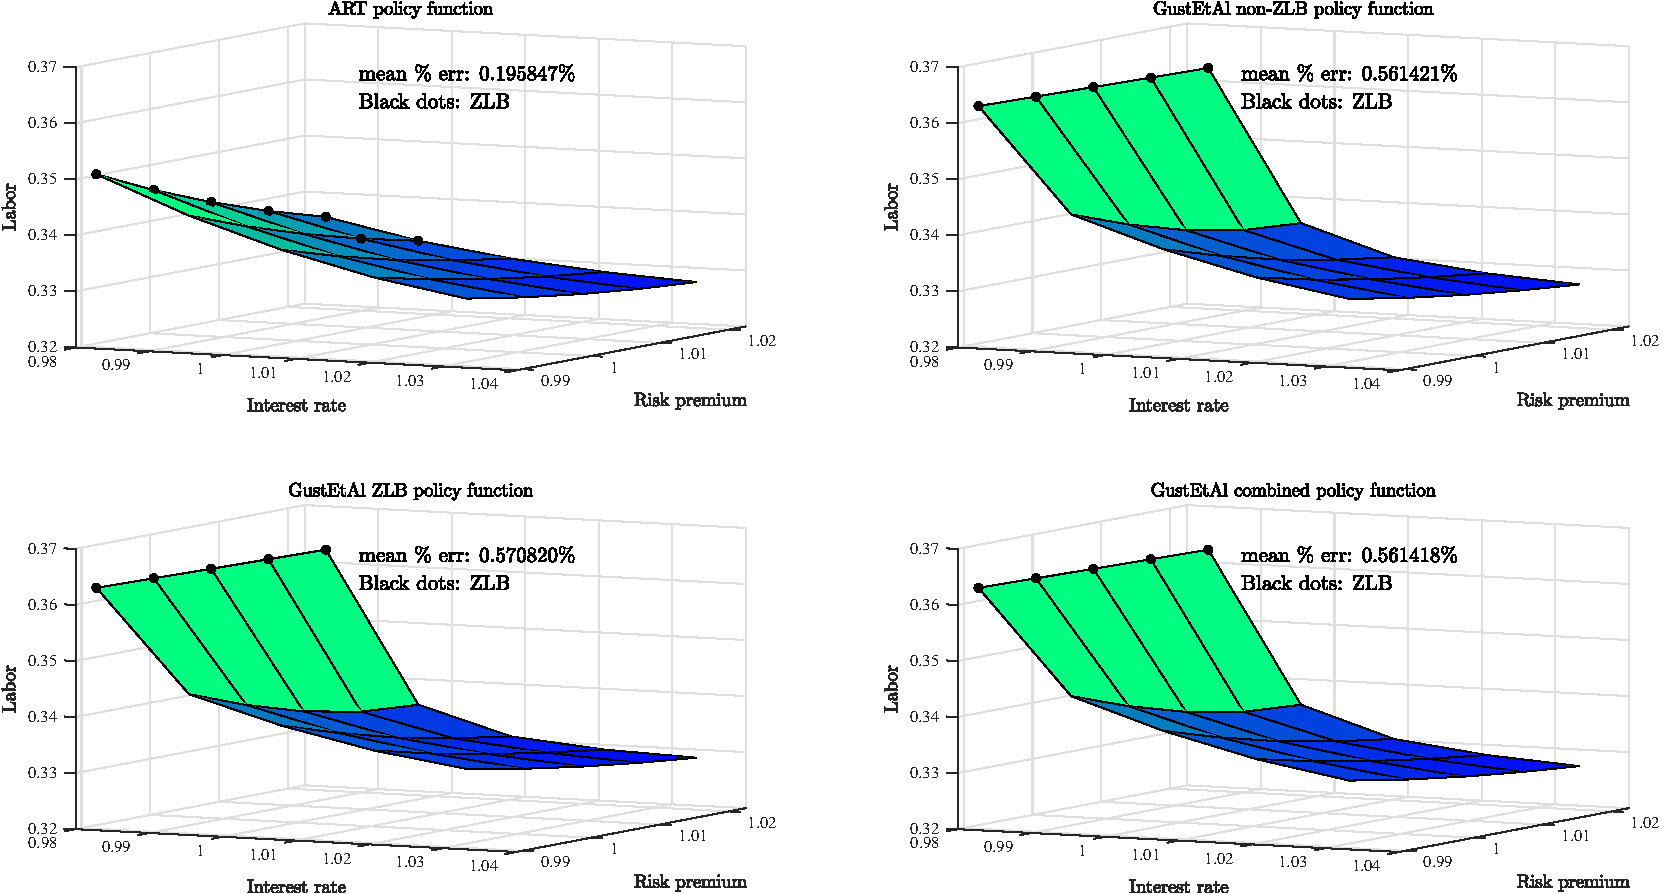
\includegraphics[scale=.6]{pfs3D_CAPITAL-eps-converted-to.pdf}%{pfs3D_CAPITAL.eps}
  \caption{Labor policy function for model with capital}    
  \label{Fig:1}
  \end{figure}

\begin{table}[H]
  \centering
  \hypertarget{Table 3}
  \small
    \setlength{\tabcolsep}{10pt}      
  \begin{tabular}{l c c c c}
    \hline
    & \multicolumn{2}{c}{Model without capital} & \multicolumn{2}{c}{Model with capital} \\
    & Mean \% Error & RMSE & Mean \% Error & RMSE\\
    \hline
    Richter et al. policy & 0.46545\% &0.0020137 consumption units & 0.19585\% & .0029035 labor units \\    
  Gust et al. policy & 0.45556\% & 0.0019792 consumption units & 0.56142\% & 0.0076665 labor units \\
  \hline
\end{tabular}
  \caption{Smoothness measures for labor policy functions ($c$ for model with capital and $n$ for model with capital). Gust et al. combined policy functions are reported.}
\end{table}
  
\subsection{Euler Equation Errors} \hyperlink{Figure 2}{Figure 2} shows the distribution of the absolute value of the Euler equation errors in base 10 logarithms for the household FOC bond, FOC capital, FOC investment, and price Phillips curve in the model with capital. We also report the mean and maximum error. The corresponding results for the model without capital is reported in \hyperlink{Appendix C}{Appendix C}.

\begin{itemize}
\item Euler equations very comparable between algorithms
\item Gust et al does slightly worse. Means are similar but max is higher.
  \end{itemize}

\begin{figure}[H]
\hypertarget{Figure 2}  
    \centering
    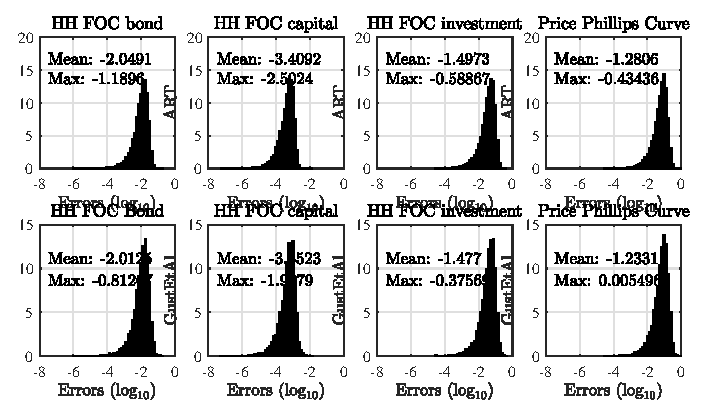
\includegraphics[scale=1.5]{eeerrors_C.eps}%{pfs3D_CAPITAL.eps}
  \caption{Euler equation errors for model with capital}    
  \end{figure}

\section{Conclusion}
% summarize results
Opportunities for future work
\begin{itemize}
\item Chebyshev polynomials
\item Smolyak grids
  \item This might make solution method faster, so we could potentially increase the number of grid points and make it better than Richter et al
  \end{itemize}

\appendix
  \section{Detrended Equilibrium System} \hypertarget{Appendix A}
  \noindent
  \textbf{Medium-Scale Model} The detrended system includes (\ref{eq:1}),(\ref{eq:6}),(\ref{eq:15}),(\ref{eq:16}) and 
\begin{gather}
\tilde{y}_t= (\tilde{k}_{t-1}/g_t)^\alpha n_t^{1-\alpha},\\
r^k_t = \alpha mc_t g_t \tilde{y}_t/\tilde{k}_{t-1},\\
\tilde{w}_t = (1-\alpha)mc_t\tilde{y}_t/n_t,\\
\tilde{y}^{gdp}_t = [1-\varphi(\pi_t^{gap} - 1)^2/2]\tilde{y}_t,\\
y^g_t = g_t\tilde{y}^{gdp}_t/(\bar{g}\tilde{y}^{gdp}_{t-1}),\\
\tilde{\lambda}_t = \tilde{c}_t\ - h\tilde{c}_{t-1}/g_t,\\
\label{eq:m1}
\tilde{w}_t = \chi n_t^\eta \tilde{\lambda}_t,\\
\tilde{c}_t + \tilde{x}_t = \tilde{y}^{gdp}_t,\\
x^g_t = g_t\tilde{x}_t/(\bar{g}\tilde{x}_{t-1}),\\
\tilde{k}_t = (1-\delta)(\tilde{k}_{t-1}/g_t) + \tilde{x}_t(1-\nu(x^g_t-1)^2/2),\\%%%
\label{eq:m2}
  1 = \beta E_t[(\tilde{\lambda}_t/\tilde{\lambda}_{t+1})(s_ti_t/(\bar{\pi}\pi_{t+1}^{gap}g_{t+1}))],\\
q_t = \beta E_t[(\tilde{\lambda}_t/\tilde{\lambda}_{t+1})(r^k_{t+1} + (1-\delta)q_{t+1})/g_{t+1}],\\
1 = q_t[1 - \nu(x^g_t-1)^2/2 - \nu(x^g_t-1)x^g_t] + \nu\beta\bar{g}E_t[q_{t+1}(\tilde{\lambda}_t/\tilde{\lambda}_{t+1})(x^g_{t+1})^2(x^g_{t+1}-1)/g_{t+1}],\\
\label{eq:m3}
  \varphi(\pi_t^{gap}-1){\pi}_t^{gap} = 1-\theta + \theta mc_t + \beta\varphi E_t[(\tilde{\lambda}_t/\tilde{\lambda}_{t+1}) (\pi_{t+1}^{gap}-1)\pi_{t+1}^{gap}(\tilde{y}_{t+1}/\tilde{y}_t)].
\end{gather}
The variables are $\tilde{c},\tilde{n},\tilde{x},\tilde{k},\tilde{y^{gdp}},\tilde{y},x^g,y^g,\tilde{w},r^k,\pi,i,i^n,q,mc,\tilde{\lambda},g,$ and $s$.\\

\noindent \textbf{Small-Scale Model} The detrended system includes (\ref{eq:1}),(\ref{eq:6}),(\ref{eq:15}),(\ref{eq:16})(\ref{eq:m1}),(\ref{eq:m2}),(\ref{eq:m3}), and 
\begin{gather}
\tilde{\lambda}_t = \tilde{c}_t,\\ %%%
\tilde{c}_t = [1-\varphi(\pi_t^{gap} - 1)^2/2]\tilde{y}_t,\\ %%%
  \tilde{y}_t= n_t.  %%% 
\end{gather}
The variables are $\tilde{c},i^n,i,\tilde{\lambda},\tilde{w},\pi^{gap},\tilde{y},n,g,$ and $s$.\\ 

\section{Nonlinear Solution Method}\hypertarget{Appendix B}
The following discussion is based on Atkinson et al. (2019) and Richter and Throckmorton (2014). We express the detrended nonlinear system compactly as
\begin{gather*}
  E[f(\textbf{s}_{t+1},\textbf{s}_t,\varepsilon_{t+1})|\textbf{z}_t,\vartheta] = 0,
\end{gather*}
where $f$ is a vector-valued function, $\textbf{s}_t$ is a vector of variables, $\varepsilon_t \equiv [\varepsilon_{s,t}, \varepsilon_{g,t},\varepsilon_{i,t}]'$ is a vector of shocks, $\textbf{z}_t$ is a vector of states ($\textbf{z}_t \equiv [\tilde{c}_{-1}, i^n_{t-1},\tilde{k}_{t-1},\tilde{x}_{t-1},s_t,g_t,\varepsilon_{i,t}]'$ for the model with capital and $\textbf{z}_t \equiv [\tilde{c}_{t-1},i^n_{t-1},s_t,g_t,\varepsilon_{i,t}]'$ for the model without capital), and $\vartheta$ is a vector of parameters.

We use the Markov chain method in Rouwenhorst (1995) to discretize the endogenous state variables, $s_t$, $g_t$, and $\varepsilon_{i,t}$ follwing Richter et al (2014). The bounds on $\tilde{c}_{t-1}, i^n_{t-1}, \tilde{k}_{t-1},$ and $\tilde{x}_{t-1}$ are set to $\pm 2.5\%, \pm 6\%, \pm 8\%, \pm 15\%$, respectively, following Atkinson et al. (2019). We discretize the states into 5 evenly-spaced points for the model with capital and 7 evenly-spaced points for the model without capital. The product of the points in each dimension, D, represents the total nodes in the state space ($D = 78125$ for the model with capital and $D = 2401$ for the model without capital). The realization of $\textbf{z}_t$ on node $d$ is denoted $\textbf{z}_t(d)$. The Rouwenhorst method provides integration nodes, $[s_{t+1}(m), g_{t+1}(m), \varepsilon_{i,t+1}(m)]$, with weights, $\phi(m)$, for $m \in \{1, \dots, M\}$.

The vector of policy functions is denoted $\textbf{pf}_t$ and the realization on node $d$ is denoted $\textbf{pf}_t(d)$ ($\textbf{pf}_t(d) \equiv [\tilde{\pi}^{gap}_t(\textbf{z}_t), n_t(\textbf{z}_t), q_t(\textbf{z}_t), mc_t(\textbf{z}_t)]$ for the model with capital and $\textbf{pf}_t(d) \equiv [\tilde{\pi}^{gap}_t(\textbf{z}_t), \tilde{c}_t(\textbf{z}_t)]$. The policy functions are selected so that solving fr other variables in the nonlinear system is straightforwards. 

The following steps outline the global policy function iteration algorithm:

\begin{enumerate}
  \item Use Sims's (2002) \texttt{gensys} algorithm to solve the log-linear model without the ZLB constraint and obtain conjectures for the policy functions $\textbf{pf}_0$.  
  \item On each node $d \in \{1,\dots,D\}$,% use fixed point iteration to find $\textbf{pf}_t(d)$ to satisfy $E[f(\cdot)|\textbf{z}_t(d), \vartheta] \approx 0$. Guess $\textbf{pf}_j(d) = \textbf{pf}_{j-1}(d)$ Then: 
    \begin{enumerate}
    \item Solve for all variables dated at time $t$, given $\textbf{pf}_t(d)$ and $\textbf{z}_t(d)$.
    \item Linearly interpolate the policy functions $\textbf{pf}_{j-1}$, at the updated state variables $\textbf{z}_{t+1}(m)$, to obtain $\textbf{pf}_{t+1}(m)$ on every integration node, $m \in \{1,\dots,M\}$.
    \item Given $\{\textbf{pf}_{t+1}(m)\}_{m=1}^M$, solve for the other elements of $\textbf{s}_{t+1}(m)$ and approximate the expectation operators %and back out the updated \textbf{pf}$_t(d)$.
      \begin{gather*}
        E[f(\textbf{s}_{t+1},\textbf{s}_t(d),\varepsilon_{t+1})|\textbf{z}_t(d),\vartheta] \approx \sum_{m=1}^M \phi(m)f(\textbf{s}_{t+1}(m),\textbf{s}_t(d),\varepsilon_{t+1}(m)).
      \end{gather*}
      \item Solve for $\textbf{pf}_t(d)$ from the expectation operators and $\textbf{s}_{t+1}(m)$. Set $\textbf{pf}_j(d) = \textbf{pf}_t(d)$.
    \end{enumerate}
       \item Repeat step 2 until $\text{maxdist}_j < 10^{-6}$, where $\text{maxdist}_j \equiv \text{max}\{|\textbf{pf}_j - \textbf{pf}_{j-1}|\}$. When that criterion is satisfied, the algorithm has converged to an approximate nonlinear solution.
\end{enumerate}

\section{Results for model without capital} \hypertarget{Appendix C}
The following reports the corresponding results for the model wtihout capital. \hyperlink{Figure 3}{Figure 3} shows the cross-section of the consumption policy functions with the interest rate and risk premium. \hyperlink{Figure 4}{Figure 4} shows the distribution of the absolute value of the Euler equation errors in base 10 logarithms for the consumption euler Equation and the price Phillips curve. 

\begin{figure}[H]
\hypertarget{Figure 3}  
    \centering
    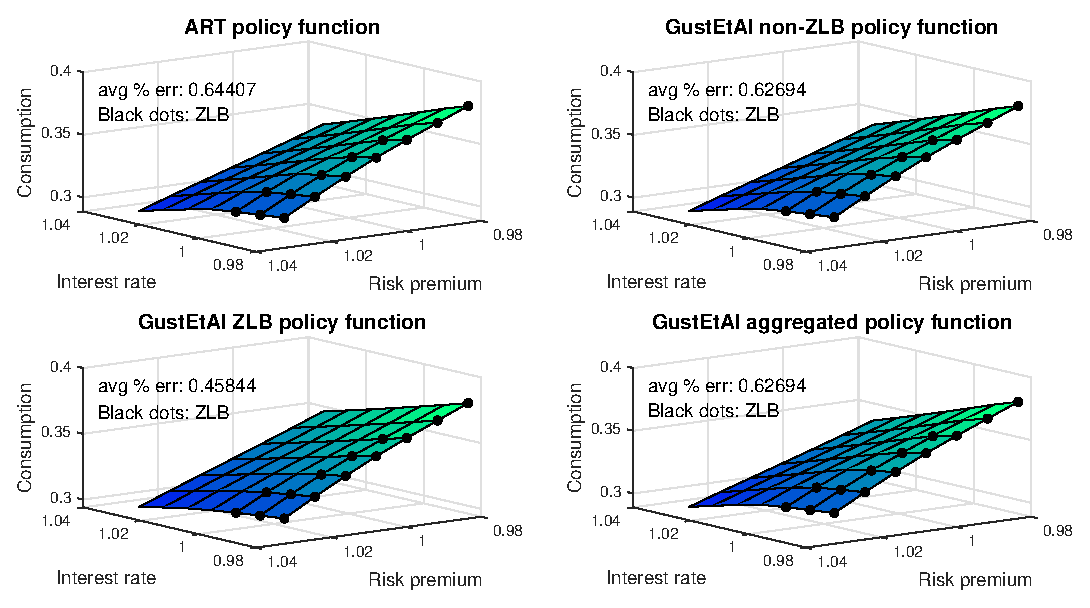
\includegraphics[scale=.6]{pfs3D.eps}
  \caption{Consumption policy function for model without capital}    
  \end{figure}

\begin{itemize}
\item Smoother in general
\item Very close between ART and GustEtAl
  \end{itemize}

\begin{figure}[H]
\hypertarget{Figure 4}  
    \centering
    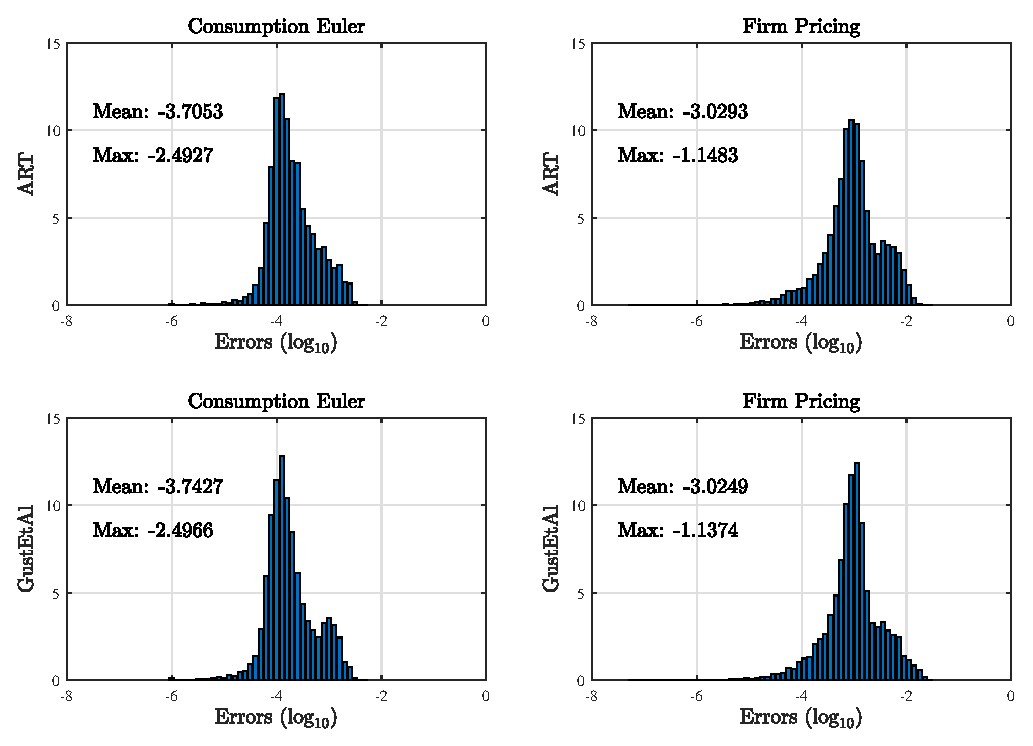
\includegraphics[scale=1.5]{eeerrors.eps}
  \caption{Euler equation errors for model without capital}    
  \end{figure}

\begin{itemize}
\item Bimodality more distinct in Gust et al policy functions
\item Very similar with regards to mean and max; Gust et al does slightly better in consumption Euler
\end{itemize}





\begin{comment}
\subsection{ART Model with capital}
\noindent Preferences:
\begin{gather*}
  E_0\textstyle\sum_{t=0}^\infty\beta^t [\log(c_t-hc^a_{t-1})-\chi n_t^{1+\eta}/(1+\eta)]
\end{gather*}

\noindent Budget Constraint:
\begin{gather*}
  c_t+x_t+b_t/(i_ts_t)=w_tn_t+r_t^kk_{t-1}+b_{t-1}/\pi_t+d_t\\
  k_t = (1-\delta)k_{t-1} + x_t(1 - \nu(x^g_t-1)^2/2)
\end{gather*}

\setcounter{equation}{0}
\noindent Equilibrium system:
\small\begin{gather}
y_t = k_{t-1}^\alpha(z_t n_t)^{1-\alpha}\\ %%%
r_t^k = \alpha mc_ty_t/k_{t-1}\\
w_t = (1-\alpha)mc_ty_t/n_t\\
%w_t^g = \pi_tw_t(\bar{\pi}gw_{t-1})\\
y_t^{gdp} = [1 - \varphi(\pi_t^{gap}-1)^2/2]y_t \\
y^g_t = y^{gdp}_t/(\bar{g}y^{gdp}_{t-1})\\
i_t^n=(i^n_{t-1})^{\rho_i}(\bar{\imath}(\pi^{gap}_t)^{\phi_\pi}(y^{g}_{t})^{\phi_y})^{1-\rho_i}\exp(mp_t)\\
i_t=\max\{1,i_t^n\}\\
\lambda_t = c_t - hc^a_{t-1} \\
w_t = \chi n_t^\eta \lambda_t\\
c_t + x_t = y_t^{gdp}\\
x_t^g = x_t/(\bar{g}x_{t-1})\\
k_t = (1-\delta)k_{t-1}+x_t(1-\nu(x_t^g-1)^2/2) \\%%%
1 =  \beta E_t[(\lambda_t/\lambda_{t+1})(s_ti_t/(\bar{\pi}\pi_{t+1}^{gap}))]\\
q_t = \beta E_t[(\lambda_t/\lambda_{t+1})(r^k_{t+1}+(1-\delta)q_{t+1})]\\
1 = q_t[1-\nu(x^g_t-1)^2/2 - \nu(x_t^g-1)x_t^g] + \nu\beta\bar{g}E_t[q_{t+1}(\lambda_t/\lambda_{t+1})(x^g_{t+1})^2(x^g_{t+1}-1)]\\
\varphi(\pi_t^{gap}-1)\pi_t^{gap} = 1-\theta + \theta mc_t + \beta\varphi E_t[(\lambda_t/\lambda_{t+1})(\pi_{t+1}^{gap}-1)\pi_{t+1}^{gap}(y_{t+1}/y_t)]\\
g_t = \bar{g} + \sigma_g\varepsilon_{g,t}\\
s_t=(1-\rho_s)\bar{s}+\rho_ss_{t-1} + \sigma_s\varepsilon_{s,t}\\
mp_t = \sigma_i\varepsilon_{i,t}\\
  z_t=g_tz_{t-1}
\end{gather}\normalsize
Variables: $\{c,n,x,k,y^{gdp},y,x^g,y^g,w,r^k,\pi,i,i^n,q,mc,\lambda,g,s,mp,z\}$\\

\setcounter{equation}{0}
\noindent De-trended Equilibrium System:
\small\begin{gather}
\tilde{y}_t= (\tilde{k}_{t-1}/g_t)^\alpha n_t^{1-\alpha}\\
r^k_t = \alpha mc_t g_t \tilde{y}_t/\tilde{k}_{t-1}\\
\tilde{w}_t = (1-\alpha)mc_t\tilde{y}_t/n_t\\
\tilde{y}^{gdp}_t = [1-\varphi(\pi_t^{gap} - 1)^2/2]\tilde{y}_t\\
y^g_t = g_t\tilde{y}^{gdp}_t/(\bar{g}\tilde{y}^{gdp}_{t-1})\\
i_t^n=(i^n_{t-1})^{\rho_i}(\bar{\imath}(\pi_t^{gap})^{\phi_\pi}(y^g_t)^{\phi_y})^{1-\rho_i}\exp(\sigma_i\varepsilon_{i,t})\\
i_t=\max\{1,i_t^n\}\\
\tilde{\lambda}_t = \tilde{c}_t\ - h\tilde{c}_{t-1}/g_t\\
\tilde{w}_t = \chi n_t^\eta \tilde{\lambda}_t  \\
\tilde{c}_t + \tilde{x}_t = \tilde{y}^{gdp}_t\\
x^g_t = g_t\tilde{x}_t/(\bar{g}\tilde{x}_{t-1})\\
\tilde{k}_t = (1-\delta)(\tilde{k}_{t-1}/g_t) + \tilde{x}_t(1-\nu(x^g_t-1)^2/2)\\%%%
  1 = \beta E_t[(\tilde{\lambda}_t/\tilde{\lambda}_{t+1})(s_ti_t/(\bar{\pi}\pi_{t+1}^{gap}g_{t+1}))]\\
q_t = \beta E_t[(\tilde{\lambda}_t/\tilde{\lambda}_{t+1})(r^k_{t+1} + (1-\delta)q_{t+1})/g_{t+1}]\\
1 = q_t[1 - \nu(x^g_t-1)^2/2 - \nu(x^g_t-1)x^g_t] + \nu\beta\bar{g}E_t[q_{t+1}(\tilde{\lambda}_t/\tilde{\lambda}_{t+1})(x^g_{t+1})^2(x^g_{t+1}-1)/g_{t+1}]\\
  \varphi(\pi_t^{gap}-1){\pi}_t^{gap} = 1-\theta + \theta mc_t + \beta\varphi E_t[(\tilde{\lambda}_t/\tilde{\lambda}_{t+1}) (\pi_{t+1}^{gap}-1)\pi_{t+1}^{gap}(\tilde{y}_{t+1}/\tilde{y}_t)]\\
  g_t= \bar{g} + \sigma_g\varepsilon_{g,t} \\
  s_t=(1-\rho_s)s_t+\rho_ss_{t-1} + \sigma_s\varepsilon_{s,t}\\
  mp_t = \sigma_i\varepsilon_{i,t}
\end{gather}
Variables:$\{\tilde{c},\tilde{n},\tilde{x},\tilde{k},\tilde{y^{gdp}},\tilde{y},x^g,y^g,\tilde{w},r^k,\pi,i,i^n,q,mc,\tilde{\lambda},g,s,mp\}$\\

\setcounter{equation}{0}
\noindent Log-linear Equilibrium System:
\begin{gather}
  \hat{y}_t/\bar{y} = \alpha(\hat{k}_{t-1}/\bar{k} - \hat{g}_t/\bar{g}) + (1-\alpha)\hat{n}_t/\bar{n}\\
\hat{r}^k_t/\bar{r}^k = \hat{mc}_t/\bar{mc} + \hat{g}_t/\bar{g} + \hat{y}_t/\bar{y} - \hat{k}_{t-1}/\bar{k}\\
\hat{w}_t/\bar{w} = \hat{mc}_t/\bar{mc} + \hat{y}_t/\bar{y} - \hat{n}_t/\bar{n}\\
\hat{y}_t^{gdp} = \hat{y}_t\\
\hat{y}^g_t = \hat{g}_t/\bar{g} + \hat{y}^{gdp}_t/\bar{y}^{gdp} - \hat{y}^{gdp}_{t-1}/\bar{y}^{gdp}\\
  \hat{i}_t/\bar{i} = \rho_i\hat{i}_{t-1}/\bar{i} + (1-\rho_i)(\phi_\pi\hat{\pi}^{gap}_t+ \phi_y\hat{y}^g_t)+\hat{mp}_t \\
  \hat{\imath}_t = \hat{\imath}_t^n\\
  \hat{\lambda}_t = \hat{c}_t - (h/\bar{g})\hat{c}_{t-1} + (h\bar{c}/\bar{g}^2)\hat{g}_t\\
  \hat{c}_t + \hat{x}_t = \hat{y}^{gdp}_t\\
  \hat{x}^g_t = \hat{g}_t/\bar{g} + \hat{x}_t/\bar{x} - \hat{x}_{t-1}/\bar{x}\\
  \hat{k}_t = ((1-\delta)/\bar{g})[\hat{k}_{t-1}-(\bar{k}/\bar{g})\hat{g}_t] + \hat{x}_t\\
  \hat{\lambda}_t/\bar{\lambda} + \hat{\imath}_t/\bar{i} + \hat{s}_t/\bar{s}  = E_t\hat{\lambda}_{t+1}/\bar{\lambda}+E_t\hat{g}_{t+1}/\bar{g}+E_t\hat{\pi}_{t+1}/\bar{\pi} \\
  \hat{q}_t = \hat{\lambda}_t/\bar{\lambda} - E_t\hat{\lambda}_{t+1}/\bar{\lambda} + (\beta/\bar{g})[E_t\hat{r}^k_{t+1} + (1-\delta)E_t\hat{q}_{t+1}] - E_t\hat{g}_{t+1}/\bar{g}\\
  \hat{x}^g_t = \hat{q}_t + \beta E_t\hat{x}^g_{t+1}\\
  \varphi\hat{\pi}^{gap}_t = \theta\hat{mc}_t+\beta\varphi E_t\hat{\pi}^{gap}_{t+1}\\
  \hat{g}_t = \sigma_g\varepsilon_{g,t}\\
  \hat{s}_t = \rho_s\hat{s}_{t-1} + \sigma_s\varepsilon_{s,t}\\
  \hat{mp}_t = \sigma_i\varepsilon_{i,t}
\end{gather}
Variables:$\{\hat{c},\hat{n},\hat{x},\hat{k},\hat{y^{gdp}},\hat{y},\hat{x^g},\hat{y^g},\hat{w},\hat{r^k},\hat{\pi},\hat{i},\hat{i^n},\hat{q},\hat{\lambda},\hat{g},\hat{s},\hat{mp}\}$\\
\begin{comment}
\pagebreak









\subsection{ART Model pre-capital}
\noindent Preferences:
\begin{gather*}
  E_0\textstyle\sum_{t=0}^\infty\beta^t [\log(c_t-hc^a_{t-1})-\chi n_t^{1+\eta}/(1+\eta)]
\end{gather*}

\noindent Budget Constraint:
\begin{gather*}
  c_t+b_t/(i_ts_t)=w_tn_t+b_{t-1}/\pi_t+d_t
\end{gather*}

\setcounter{equation}{0}
\noindent Equilibrium system (11 equations):
\small\begin{gather}
c_t = [1-\varphi(\pi_t^{gap}-1)^2/2]y_t\\
i_t^n=(i^n_{t-1})^{\rho_i}(\bar{\imath}(\pi^{gap}_t)^{\phi_\pi}(c_t/(\bar{g}c_{t-1}))^{\phi_c})^{1-\rho_i}\exp(\sigma_\nu\nu_t)\\
i_t=\max\{1,i_t^n\}\\
\lambda_t = c_t - hc^a_{t-1} \\
w_t = \chi n_t^\eta \lambda_t\\
1 =  \beta E_t[(\lambda_t/\lambda_{t+1})(s_ti_t/(\bar{\pi}\pi_{t+1}^{gap}))]\\
\varphi(\pi_t^{gap}-1)\pi_t^{gap} = 1-\theta + \theta w_t/z_t + \beta\varphi E_t[(\lambda_t/\lambda_{t+1})(\pi_{t+1}^{gap}-1)\pi_{t+1}^{gap}(y_{t+1}/y_t)]\\
  y_t=z_t n_t\\  
  g_t= (1-\rho_g)\bar{g}+\rho_gg_{t-1} + \sigma_\varepsilon\varepsilon_t \\
  s_t=(1-\rho_s)\bar{s}+\rho_ss_{t-1} + \sigma_\upsilon\upsilon_t\\
  z_t=g_tz_{t-1}
\end{gather}\normalsize
Variables: $\{c,i^n,i,\lambda,w,\pi^{gap},y,n,g,s,z\}$\\

\setcounter{equation}{0}
\noindent De-trended Equilibrium System (10 equations):
\small\begin{gather}
\tilde{c}_t = [1-\varphi(\pi_t^{gap} - 1)^2/2]\tilde{y}_t\\
i_t^n=(i^n_{t-1})^{\rho_i}(\bar{\imath}(\pi_t^{gap})^{\phi_\pi}(g_t\tilde{c}_t/(\bar{g}\tilde{c}_{t-1})^{\phi_c})^{1-\rho_i}\exp(\sigma_\nu\nu_t)\\
i_t=\max\{1,i_t^n\}\\
\tilde{\lambda}_t = \tilde{c}_t\ - h\tilde{c}_{t-1}/g_t\\
\tilde{w}_t = \chi n_t^\eta \tilde{\lambda}_t  \\
  1 = \beta E_t[(\tilde{\lambda}_t/\tilde{\lambda}_{t+1})(s_ti_t/(\bar{\pi}\pi_{t+1}^{gap}g_{t+1}))]\\
  \varphi(\pi_t^{gap}-1){\pi}_t^{gap} = 1-\theta + \theta\tilde{w}_t + \beta\varphi E_t[(\tilde{\lambda}_t/\tilde{\lambda}_{t+1}) (\pi_{t+1}^{gap}-1)\pi_{t+1}^{gap}(\tilde{y}_{t+1}/\tilde{y}_t)]\\
  \tilde{y}_t= n_t\\  
  g_t= (1-\rho_g)\bar{g}+\rho_gg_{t-1} + \sigma_\varepsilon\varepsilon_t \\
  s_t=(1-\rho_s)s_t+\rho_ss_{t-1} + \sigma_\upsilon\upsilon_t
\end{gather}
Variables: $\{\tilde{c},i^n,i,\tilde{\lambda},\tilde{w},\pi^{gap},\tilde{y},n,k,g,s\}$\\ 

\setcounter{equation}{0}
\noindent Log-linear Equilibrium System:
\begin{gather}
  \hat{c}_t = \hat{y}_t\\
  \hat{\imath}_t^n = \rho_i\hat{\imath}^n_{t-1} + (1-\rho_i)\phi_\pi\hat{\pi}_t+ (1-\rho_i)\phi_c(\hat{g}+\hat{c}-\hat{c}_{t-1})+\sigma_\nu\nu_t \\
  \hat{\imath}_t = \hat{\imath}_t^n\\
  (1-h/g)\hat{\lambda}_t = \hat{c}_t + (h/g)(\hat{g} - \hat{c}_{t-1})\\
  \hat{w}_t =  \eta\hat{n}_t + \hat{\lambda}_t\\
  \hat{\lambda}_t + \hat{\imath}_t + s_t  = E_t\hat{\lambda}_{t+1}+E_t\hat{\pi}_{t+1} \\
  \varphi\hat{\pi}_t = (\theta-1)\hat{w}_t+\beta\varphi E_t\hat{\pi}_{t+1}\\
  \hat{y}_t = \hat{n}_t 
\end{gather}
\pagebreak
\setcounter{equation}{0}
\subsection{Gust Et Al Model}
\noindent Equilibrium system (13 equations):
\small\begin{gather}
\varphi(\pi_t^{gap}-1)\pi_t^{gap} = 1-\theta + \theta w_t/z_t + \beta\varphi E_t[(\lambda_t/\lambda_{t+1})(\pi_{t+1}^{gap}-1)\pi_{t+1}^{gap}(y_{t+1}/y_t)]\\
i_t^n=(i^n_{t-1})^{\rho_i}(\bar{\imath}(\pi^{gap}_t)^{\phi_\pi})^{1-\rho_i}\exp(\sigma_\nu\nu_t)\\
i_t=\max\{1,i_t^n\}\\
1/\lambda_t =  \beta E_t[(1/\lambda_{t+1})(s_ti_t/(\bar{\pi}\pi_{t+1}^{gap}g_{t+1}))]\\
\lambda_t = c_t \\
c_t = [1-\varphi(\pi_t^{gap}-1)^2/2]y_t\\
w_t = \chi n_t^\eta \lambda_t\\
  y_t=z_t n_t\\  
  g_t= (1-\rho_g)\bar{g}+\rho_gg_{t-1} + \sigma_\varepsilon\varepsilon_t \\
  s_t=(1-\rho_s)\bar{s}+\rho_ss_{t-1} + \sigma_\upsilon\upsilon_t\\
  z_t=g_tz_{t-1}
\end{gather}\normalsize
Variables: $\{c,i^n,i,\lambda,w,\pi^{gap},V_{\lambda},y,V_{\pi},n,g,s,z\}$\\

\setcounter{equation}{0}
\noindent De-trended Equilibrium System (12 equations):
\small\begin{gather}
\varphi(\pi_t^{gap}-1){\pi}_t^{gap} = 1 - \theta + \theta\tilde{w}_t + \beta\varphi E_t[(\tilde{\lambda}_t/\tilde{\lambda}_{t+1})(\pi^{gap}_{t+1}-1)\pi^{gap}_{t+1}(\tilde{y}_{t+1}/\tilde{y}_t)]\\
i_t^n=(i^n_{t-1})^{\rho_i}(\bar{\imath}(\pi_t^{gap})^{\phi_\pi})^{1-\rho_i}\exp(\sigma_\nu\nu_t)\\
i_t=\max\{1,i_t^n\}\\
1/\tilde{\lambda}_t = \beta E_t[(1/\tilde{\lambda}_{t+1})(s_ti_t/(\bar{\pi}\pi^{gap}_{t+1}g_{t+1}))]\\%
\tilde{\lambda}_t = \tilde{c}_t\\
\tilde{c}_t = [1-\varphi(\pi_t^{gap} - 1)^2/2]\tilde{y}_t\\
\tilde{w}_t = \chi n_t^\eta \tilde{\lambda}_t  \\
  \tilde{y}_t= n_t\\  
  g_t= (1-\rho_g)\bar{g}+\rho_gg_{t-1} + \sigma_\varepsilon\varepsilon_t \\
  s_t=(1-\rho_s)s_t+\rho_ss_{t-1} + \sigma_\upsilon\upsilon_t
\end{gather}
Variables: $\{\tilde{c},i^n,i,\tilde{\lambda},\tilde{w},\pi^{gap},\tilde{V}_{\lambda},\tilde{y},\tilde{V}_{\pi},n,g,s\}$\\ 

\setcounter{equation}{0}
\noindent Log-linear Equilibrium System:
\begin{gather}
  \varphi\hat{\pi}_t = (\theta-1)\hat{w}_t+\beta\varphi E_t\hat{\pi}_{t+1}\\
  \hat{\imath}_t^n = \rho_i\hat{\imath}^n_{t-1} + (1-\rho_i)\phi_\pi\hat{\pi}_t+\sigma_\nu\nu_t \\
  \hat{\imath}_t = \hat{\imath}_t^n\\
    -\hat{\lambda}_t = \hat{\imath}_t + s_t - E_t\hat{\lambda}_{t+1} - E_t\hat{\pi}_{t+1} \\
  \hat{\lambda}_t = \hat{c}_t \\
  \hat{c}_t = \hat{y}_t\\
  \hat{w}_t =  \eta\hat{n}_t + \hat{\lambda}_t\\
  \hat{y}_t = \hat{n}_t
\end{gather}

\setcounter{equation}{0}
\noindent Gust et al Indicator Functions\\
\begin{gather}
  c_{t+1,1} = \beta E_t[\lambda_t(s_ti_t/(\bar{\pi}\pi_{t+1}^{gap}g_{t+1}))]\\
  c_{t+1,2} = \beta E_t[\lambda_t(s_t/(\bar{\pi}\pi_{t+1}^{gap}g_{t+1}))]\\  
\end{gather}
for $k=1,2$ where $k=1$ corresponds to the non-ZLB regime and $k=2$ corresponds to the ZLB regime.
\begin{gather}
c_{t} = c_{t,1}I + c_{t,2}(1-I) 
\end{gather}
for $j=1,2$ and where $I$ is defined by:
$$
\begin{cases}
  I = 1 & \text{ if } i > 1\\
  I = 0 & \text{ otherwise.}
\end{cases}
$$
%We use the functions, $V_l$, to determine the decisions rule though we do not approximate $V_l$ directly, because they inherit a kink associated with the ZLB constraint. Instead, we approximate functions, $V_{l,i}$, that are smoother and easier to approximate by specifying:
%\begin{gather}
%V_l = V_{l,1}I + V_{l,2}(1-I) 
%\end{gather}
%for $l \in \{\lambda, \pi\}$ and $j=1,2$ and where $I$ is defined by:
%\begin{gather}
%  I = 1 \text{ if } i > 1\\
%  \text{  } = 0 \text{ otherwise}
%\end{gather}
%In the above, $i = \max(1,i^n)$ where $i^n$ denotes the value of the notional rate derived from evaluating the functions $V_{l,1}$ and using (2). (For each variable, we use $j=1$ to denote the function associated with the regime with a positive nominal interest rate and $j=2$ to denote the function associated with the ZLB regime. \\
%Because the functions, $V_l$ depend directly on the nominal interest rate, we expect then to have a kink or non-differentiability. By contrast, the counterpart functions, $V_{l,j}$, that are indexed by the interest-rate regime do not depend on the current indicator function and thus are more likely to be smooth. \\
%Specifically, $V_{\pi,1}$ and $V_{\pi,2}$ are both described by (8) because the nominal interest rate does not appear in that equation. $V_{\lambda,1}$ is described by (6), but for the ZLB regime:
%\begin{gather}
%V_{\lambda,t,2} =  \beta E_t[(1/\lambda_{t+1})(s_t/(\bar{\pi}\pi_{t+1}^{gap}g_{t+1}))]\\  
%\end{gather}
%where $i_t$ is replaced by 1.
\end{comment}
\end{document}

\documentclass[12pt, final]{article}
\usepackage{color}
\usepackage{times}
\usepackage{amssymb,amsmath,amsthm}
\usepackage{dsfont}
\usepackage{graphicx}
\usepackage{enumerate}
\usepackage{enumitem}
\usepackage[paperwidth=8.5in,left=1.0in,right=1.0in,top=1.0in,bottom=1.0in,paperheight=11.0in]{geometry}
\usepackage[labelsep=colon,singlelinecheck=false,footnotesize]{caption}
\usepackage{fancyhdr}
\usepackage{float}
\usepackage{booktabs}
\usepackage[sort&compress]{natbib}
\usepackage{subfig}
\usepackage{titlesec}
\usepackage[breaklinks]{hyperref}
\hypersetup{pdfdisplaydoctitle=true,bookmarksnumbered=true,colorlinks=true,citecolor=black,linkcolor=darkblue,urlcolor=darkred,pdfstartview=FitH,pdfpagemode=UseNone}
\usepackage[hyphenbreaks]{breakurl}
\usepackage{accents}
\newcommand{\ubar}[1]{\underaccent{\bar}{#1}}


%Define Color Names
\definecolor{Gray}{rgb}{0.65,0.65,0.65}
\definecolor{darkblue}{rgb}{0,0,0.55}
\definecolor{darkred}{rgb}{0.5,0,0}

%Section Headings
\newcommand\Bheadfont{\fontsize{14pt}{\baselineskip}\selectfont}
\titleformat{\section}[hang]{\normalfont\sc\color{darkblue}\Bheadfont}{\thesection\hskip0.618em}{0em}{}
\titlespacing*{\section}{0pt}{15pt plus 2pt minus 2pt}{9pt plus 2pt minus 2pt}
\titleformat{\subsection}[runin]{\normalfont\sc\color{darkblue}} {\thesubsection\hskip0.618em}{0em}{}
\titlespacing*{\subsection}{0pt}{13pt plus 2pt minus 2pt}{13pt plus 2pt minus 2pt}
\titleformat{\subsubsection}[runin]{\normalfont\sc\color{darkblue}} {\thesubsubsection\hskip0.618em}{0em}{}
\titlespacing*{\subsubsection}{0pt}{13pt plus 2pt minus 2pt}{13pt plus 2pt minus 2pt}
\titleformat{\paragraph}[runin]{\bfseries}{\theparagraph\hskip0.618em}{0em}{}
\titlespacing*{\paragraph}{0pt}{13pt plus 2pt minus 2pt}{13pt plus 2pt minus 2pt}

\begin{document}

\section{Equilibrium System}

\noindent Preferences:
\begin{gather*}
  E_0\textstyle\sum_{t=0}^\infty\beta^t [\log(c_t)-\chi n_t^{1+\eta}/(1+\eta)]
\end{gather*}

\noindent Budget Constraint:
\begin{gather*}
  c_t+b_t/(i_ts_t)=w_tn_t+b_{t-1}/\pi_t+d_t
\end{gather*}

\setcounter{equation}{0}
\subsection{ART Model}
\noindent Equilibrium system (11 equations):
\small\begin{gather}
c_t = [1-\varphi(\pi_t^{gap}-1)^2/2]y_t\\
i_t^*=(i^*_{t-1})^{\rho_i}(\bar{\imath}(\pi^{gap}_t)^{\phi_\pi})^{1-\rho_i}\exp(\sigma_\nu\nu_t)\\
i_t=\max\{1,i_t^*\}\\
\lambda_t = c_t \\
w_t = \chi n_t^\eta \lambda_t\\
1 =  \beta E_t[(\lambda_t/\lambda_{t+1})(s_ti_t/(\bar{\pi}\pi_{t+1}^{gap}g_{t+1}))]\\
\varphi(\pi_t^{gap}-1)\pi_t^{gap} = 1-\theta + \theta w_t/z_t + \beta\varphi E_t[(\lambda_t/\lambda_{t+1})(\pi_{t+1}^{gap}-1)\pi_{t+1}^{gap}(y_{t+1}/y_t)]\\
  y_t=z_t n_t\\  
  g_t= (1-\rho_g)\bar{g}+\rho_gg_{t-1} + \sigma_\varepsilon\varepsilon_t \\
  s_t=(1-\rho_s)\bar{s}+\rho_ss_{t-1} + \sigma_\upsilon\upsilon_t\\
  z_t=g_tz_{t-1}
\end{gather}\normalsize
Variables: $\{c,i^*,i,\lambda,w,\pi^{gap},y,n,g,s,z\}$\\

\setcounter{equation}{0}
\noindent De-trended Equilibrium System (10 equations):
\small\begin{gather}
\tilde{c}_t = [1-\varphi(\pi_t^{gap} - 1)^2/2]\tilde{y}_t\\
i_t^*=(i^*_{t-1})^{\rho_i}(\bar{\imath}(\pi_t^{gap})^{\phi_\pi})^{1-\rho_i}\exp(\sigma_\nu\nu_t)\\
i_t=\max\{1,i_t^*\}\\
\tilde{\lambda}_t = \tilde{c}_t\\
\tilde{w}_t = \chi n_t^\eta \tilde{\lambda}_t  \\
  1 = \beta E_t[(\tilde{\lambda}_t/\tilde{\lambda}_{t+1})(s_ti_t/(\bar{\pi}\pi_{t+1}^{gap}g_{t+1}))]\\
  \varphi(\pi_t^{gap}-1){\pi}_t^{gap} = 1-\theta + \theta\tilde{w}_t + \beta\varphi E_t[(\tilde{\lambda}_t/\tilde{\lambda}_{t+1}) (\pi_{t+1}^{gap}-1)\pi_{t+1}^{gap}(\tilde{y}_{t+1}/\tilde{y}_t)]\\
  \tilde{y}_t= n_t\\  
  g_t= (1-\rho_g)\bar{g}+\rho_gg_{t-1} + \sigma_\varepsilon\varepsilon_t \\
  s_t=(1-\rho_s)s_t+\rho_ss_{t-1} + \sigma_\upsilon\upsilon_t
\end{gather}
Variables: $\{\tilde{c},i^*,i,\tilde{\lambda},\tilde{w},\pi^{gap},\tilde{y},n,g,s\}$\\ 

\setcounter{equation}{0}
\noindent Log-linear Equilibrium System:
\begin{gather}
  \hat{c}_t = \hat{y}_t\\
  \hat{\imath}_t^n = \rho_i\hat{\imath}^n_{t-1} + (1-\rho_i)\phi_\pi\hat{\pi}_t+\sigma_\nu\nu_t \\
  \hat{\imath}_t = \hat{\imath}_t^n\\
  \hat{\lambda}_t = \hat{c}_t \\
  \hat{w}_t =  \eta\hat{n}_t + \hat{\lambda}_t\\
  \hat{\lambda}_t + \hat{\imath}_t + s_t  = E_t\hat{\lambda}_{t+1}+E_t\hat{\pi}_{t+1} \\
  \varphi\hat{\pi}_t = (\theta-1)\hat{w}_t+\beta\varphi E_t\hat{\pi}_{t+1}\\
  \hat{y}_t = \hat{n}_t 
\end{gather}
\pagebreak
\setcounter{equation}{0}
\subsection{Gust Et Al Model}
\noindent Equilibrium system (13 equations):
\small\begin{gather}
\varphi(\pi_t^{gap}-1)\pi_t^{gap} = 1-\theta + \theta w_t/z_t + \beta\varphi E_t[(\lambda_t/\lambda_{t+1})(\pi_{t+1}^{gap}-1)\pi_{t+1}^{gap}(y_{t+1}/y_t)]\\
i_t^*=(i^*_{t-1})^{\rho_i}(\bar{\imath}(\pi^{gap}_t)^{\phi_\pi})^{1-\rho_i}\exp(\sigma_\nu\nu_t)\\
i_t=\max\{1,i_t^*\}\\
1/\lambda_t =  \beta E_t[(1/\lambda_{t+1})(s_ti_t/(\bar{\pi}\pi_{t+1}^{gap}g_{t+1}))]\\
\lambda_t = c_t \\
c_t = [1-\varphi(\pi_t^{gap}-1)^2/2]y_t\\
w_t = \chi n_t^\eta \lambda_t\\
  y_t=z_t n_t\\  
  g_t= (1-\rho_g)\bar{g}+\rho_gg_{t-1} + \sigma_\varepsilon\varepsilon_t \\
  s_t=(1-\rho_s)\bar{s}+\rho_ss_{t-1} + \sigma_\upsilon\upsilon_t\\
  z_t=g_tz_{t-1}
\end{gather}\normalsize
Variables: $\{c,i^*,i,\lambda,w,\pi^{gap},V_{\lambda},y,V_{\pi},n,g,s,z\}$\\

\setcounter{equation}{0}
\noindent De-trended Equilibrium System (12 equations):
\small\begin{gather}
\varphi(\pi_t^{gap}-1){\pi}_t^{gap} = 1 - \theta + \theta\tilde{w}_t + \beta\varphi E_t[(\tilde{\lambda}_t/\tilde{\lambda}_{t+1})(\pi^{gap}_{t+1}-1)\pi^{gap}_{t+1}(\tilde{y}_{t+1}/\tilde{y}_t)]\\
i_t^*=(i^*_{t-1})^{\rho_i}(\bar{\imath}(\pi_t^{gap})^{\phi_\pi})^{1-\rho_i}\exp(\sigma_\nu\nu_t)\\
i_t=\max\{1,i_t^*\}\\
1/\tilde{\lambda}_t = \beta E_t[(1/\tilde{\lambda}_{t+1})(s_ti_t/(\bar{\pi}\pi^{gap}_{t+1}g_{t+1}))]\\%
\tilde{\lambda}_t = \tilde{c}_t\\
\tilde{c}_t = [1-\varphi(\pi_t^{gap} - 1)^2/2]\tilde{y}_t\\
\tilde{w}_t = \chi n_t^\eta \tilde{\lambda}_t  \\
  \tilde{y}_t= n_t\\  
  g_t= (1-\rho_g)\bar{g}+\rho_gg_{t-1} + \sigma_\varepsilon\varepsilon_t \\
  s_t=(1-\rho_s)s_t+\rho_ss_{t-1} + \sigma_\upsilon\upsilon_t
\end{gather}
Variables: $\{\tilde{c},i^*,i,\tilde{\lambda},\tilde{w},\pi^{gap},\tilde{V}_{\lambda},\tilde{y},\tilde{V}_{\pi},n,g,s\}$\\ 

\setcounter{equation}{0}
\noindent Log-linear Equilibrium System:
\begin{gather}
  \varphi\hat{\pi}_t = (\theta-1)\hat{w}_t+\beta\varphi E_t\hat{\pi}_{t+1}\\
  \hat{\imath}_t^n = \rho_i\hat{\imath}^n_{t-1} + (1-\rho_i)\phi_\pi\hat{\pi}_t+\sigma_\nu\nu_t \\
  \hat{\imath}_t = \hat{\imath}_t^n\\
    -\hat{\lambda}_t = \hat{\imath}_t + s_t - E_t\hat{\lambda}_{t+1} - E_t\hat{\pi}_{t+1} \\
  \hat{\lambda}_t = \hat{c}_t \\
  \hat{c}_t = \hat{y}_t\\
  \hat{w}_t =  \eta\hat{n}_t + \hat{\lambda}_t\\
  \hat{y}_t = \hat{n}_t
\end{gather}

\setcounter{equation}{0}
\noindent Gust et al Indicator Functions\\
\begin{gather}
  c_{t+1,1} = \beta E_t[\lambda_t(s_ti_t/(\bar{\pi}\pi_{t+1}^{gap}g_{t+1}))]\\
  c_{t+1,2} = \beta E_t[\lambda_t(s_t/(\bar{\pi}\pi_{t+1}^{gap}g_{t+1}))]\\  
\end{gather}
for $k=1,2$ where $k=1$ corresponds to the non-ZLB regime and $k=2$ corresponds to the ZLB regime.
\begin{gather}
c_{t} = c_{t,1}I + c_{t,2}(1-I) 
\end{gather}
for $j=1,2$ and where $I$ is defined by:
$$
\begin{cases}
  I = 1 & \text{ if } i > 1\\
  I = 0 & \text{ otherwise.}
\end{cases}
$$
%We use the functions, $V_l$, to determine the decisions rule though we do not approximate $V_l$ directly, because they inherit a kink associated with the ZLB constraint. Instead, we approximate functions, $V_{l,i}$, that are smoother and easier to approximate by specifying:
%\begin{gather}
%V_l = V_{l,1}I + V_{l,2}(1-I) 
%\end{gather}
%for $l \in \{\lambda, \pi\}$ and $j=1,2$ and where $I$ is defined by:
%\begin{gather}
%  I = 1 \text{ if } i > 1\\
%  \text{  } = 0 \text{ otherwise}
%\end{gather}
%In the above, $i = \max(1,i^*)$ where $i^*$ denotes the value of the notional rate derived from evaluating the functions $V_{l,1}$ and using (2). (For each variable, we use $j=1$ to denote the function associated with the regime with a positive nominal interest rate and $j=2$ to denote the function associated with the ZLB regime. \\
%Because the functions, $V_l$ depend directly on the nominal interest rate, we expect then to have a kink or non-differentiability. By contrast, the counterpart functions, $V_{l,j}$, that are indexed by the interest-rate regime do not depend on the current indicator function and thus are more likely to be smooth. \\
%Specifically, $V_{\pi,1}$ and $V_{\pi,2}$ are both described by (8) because the nominal interest rate does not appear in that equation. $V_{\lambda,1}$ is described by (6), but for the ZLB regime:
%\begin{gather}
%V_{\lambda,t,2} =  \beta E_t[(1/\lambda_{t+1})(s_t/(\bar{\pi}\pi_{t+1}^{gap}g_{t+1}))]\\  
%\end{gather}
%where $i_t$ is replaced by 1.
\end{comment}
\end{document}

